\documentclass{article}
\usepackage{tikz}
\usetikzlibrary{arrows.meta}

\begin{document}

\begin{figure}[h]
    \centering
    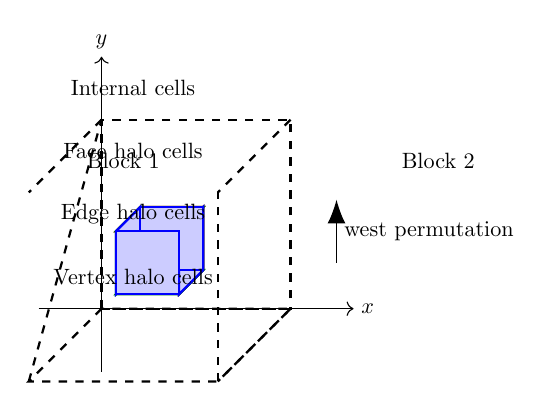
\begin{tikzpicture}[scale=0.8, every node/.style={scale=0.8}]
        % Define colors
        \definecolor{redColor}{RGB}{255,0,0}
        \definecolor{greenColor}{RGB}{0,128,0}
        \definecolor{blueColor}{RGB}{0,0,255}
        
        % Draw the coordinate system
        \draw[->] (-1,0,0) -- (4,0,0) node[right] {$x$};
        \draw[->] (0,-1,0) -- (0,4,0) node[above] {$y$};
        
        % Draw the blocks
        \draw[dashed, thick] (0,0,0) -- (3,0,0) -- (3,3,0) -- (0,3,0) -- cycle;
        \draw[dashed, thick] (0,0,0) -- (0,0,3) -- (3,0,3) -- (3,0,0) -- cycle;
        \draw[dashed, thick] (0,0,0) -- (0,3,0);
        \draw[dashed, thick] (0,0,3) -- (0,3,0);
        \draw[dashed, thick] (3,0,0) -- (3,0,3);
        \draw[dashed, thick] (3,3,0) -- (3,3,3);
        \draw[dashed, thick] (0,3,0) -- (0,3,3);
        \draw[dashed, thick] (3,0,3) -- (3,3,3);
        
        % Draw the halo cells
        \draw[redColor, thick, fill=redColor!20] (1,1,1) -- (2,1,1) -- (2,2,1) -- (1,2,1) -- cycle;
        \draw[redColor, thick, fill=redColor!20] (1,1,2) -- (2,1,2) -- (2,2,2) -- (1,2,2) -- cycle;
        \draw[redColor, thick, fill=redColor!20] (1,2,1) -- (2,2,1) -- (2,2,2) -- (1,2,2) -- cycle;
        \draw[redColor, thick, fill=redColor!20] (2,1,1) -- (2,2,1) -- (2,2,2) -- (2,1,2) -- cycle;
        
        \draw[greenColor, thick, fill=greenColor!20] (1,1,1) -- (1,2,1) -- (1,2,2) -- (1,1,2) -- cycle;
        \draw[greenColor, thick, fill=greenColor!20] (2,1,1) -- (2,2,1) -- (2,2,2) -- (2,1,2) -- cycle;
        \draw[greenColor, thick, fill=greenColor!20] (1,1,1) -- (1,1,2) -- (2,1,2) -- (2,1,1) -- cycle;
        \draw[greenColor, thick, fill=greenColor!20] (1,2,1) -- (1,2,2) -- (2,2,2) -- (2,2,1) -- cycle;
        
        \draw[blueColor, thick, fill=blueColor!20] (1,1,1) -- (1,1,2) -- (1,2,2) -- (1,2,1) -- cycle;
        \draw[blueColor, thick, fill=blueColor!20] (2,1,1) -- (2,1,2) -- (2,2,2) -- (2,2,1) -- cycle;
        \draw[blueColor, thick, fill=blueColor!20] (1,1,1) -- (1,2,1) -- (2,2,1) -- (2,1,1) -- cycle;
        \draw[blueColor, thick, fill=blueColor!20] (1,1,2) -- (1,2,2) -- (2,2,2) -- (2,1,2) -- cycle;
        
        % Block labels
        \node at (1.5,3.5,3) {Block 1};
        \node at (6.5,3.5,3) {Block 2};
        
        % Arrows and labels
        \draw[-{Latex[length=3mm]}] (4.5,1.5,2) -- (4.5,2.5,2) node[midway, right] {west permutation};
        
        % Text labels
        \node at (0.5,0.5,0) {Vertex halo cells};
        \node at (0.5,1.5,0) {Edge halo cells};
        \node at (0.5,2.5,0) {Face halo cells};
        \node at (0.5,3.5,0) {Internal cells};
    \end{tikzpicture}
    \caption{Schematic illustration of two adjacent blocks in $x$-direction within the homogeneous domain decomposition during a halo update. Depicted are the face (blue), edge (green), and vertex (red) halo cells of block 1 at the east side of the block. We highlight the corresponding cells in block 2 that are required for the halo update accordingly. This update entails a west permutation, i.e., a permutation of data from block 2 to block 1.}
    \label{fig:block_halo_update}
\end{figure}

\end{document}